\documentclass[10pt,a4paper,danish]{article}
%% Indlæs ofte brugte pakker
\usepackage{amssymb}
\usepackage[danish]{babel}
\usepackage[utf8]{inputenc}
\usepackage{listings}
\usepackage{fancyhdr}
\usepackage{hyperref}
\usepackage{booktabs}
\usepackage{graphicx}
\usepackage{todonotes}
\usepackage{algorithmic}
\usepackage{amsmath}

\pagestyle{fancy}
\fancyhead{}
\fancyfoot{}
\rhead{\today}
\rfoot{\thepage}
\setlength{\parindent}{0pt}

% Opsæt indlæsning af filer
\lstset{
 language=Python,
 extendedchars=\true,
 inputencoding=utf8,
 linewidth=\textwidth, basicstyle=\small,
 numbers=left, numberstyle=\footnotesize,
 tabsize=2, showstringspaces=false,
 breaklines=true, breakatwhitespace=false,
}

%% Titel og forfatter
\title{G3\\Maskinarkitektur\\Efterår 2011}
\author{Jens Fredskov\\ Naja Mottelson\\Søren Pilgård}

%% Start dokumentet
\begin{document}

%% Vis titel
\maketitle
\newpage

%% Vis indholdsfortegnelse
\tableofcontents
\newpage

%% Klar, parat, start!
\section{Indledning}
Denne rapport dokumenterer gruppens arbejde med tredje godkendelsesopgave i kurset 
Maskinarkitektur. Begge de udleverede afprøvningsprogrammer kører på
arkitekturen, og giver de rigtige resultater (ift. til de kommentarerer som
programmerne indeholder). Derudoverer arkitekturen afprøvet ved at lade vores
program fra G2.2 (et program der udregner den længeste vej -- se evt. det
vedlagte program).

\paragraph{}
I nærværende rapport har vi valgt at fokusere på at beskrive de punkter på 
hvilke vores implementering adskiller sig fra det man kan finde i lærebogen -- 
de steder hvor vi har valgt at følge bogens tilgang er derfor som udgangspunkt
ikke beskrevet her. Dette omfatter implementeringen af de aritmetisk-logiske
instruktioner samt implementeringen af selve pipeline-registrene.  

\paragraph{}
Af overordnede afvigelser fra lærebogen kan nævnes vores valg mht. indeksering:
Imellem hver pipeline videresender vi PC + 4 i stedet for PC. Dette sparer os 
for at trække 4 fra PC'en ved hopforudsigelsestabellen. 

\paragraph{}

\section{Fremsendingsenhed}
Vores implementering af kredsløbets fremsendingsenhhed (se Figur \ref{fig:fu}) er 
en direkte oversættelse af den pseudokode der er at finde i lærebogen (s. 369)
-- dog med de rettelser der er at finde i opgaveformuleringen. 

\paragraph{}
Ved undersøgelse for datafarer i MEM-stadiet undersøges der først 
for hvorvidt MEM/WB.RegWrite er sat, og at destinationsregistret
ikke er \$0. Hvis dette er tilfældet sammenlignes destinationsregistret
med hhv. rs- og rt-registrene i ID/EX (hvis en lighed findes har vi en 
datafare). Logikken for undersøgelse for EX-datafarer er implementeret
på samme vis, og ført igennem en NOT-gate for at lede til det endegyldige
udtryk. 

\begin{figure}[htb]
\begin{center}
\leavevmode
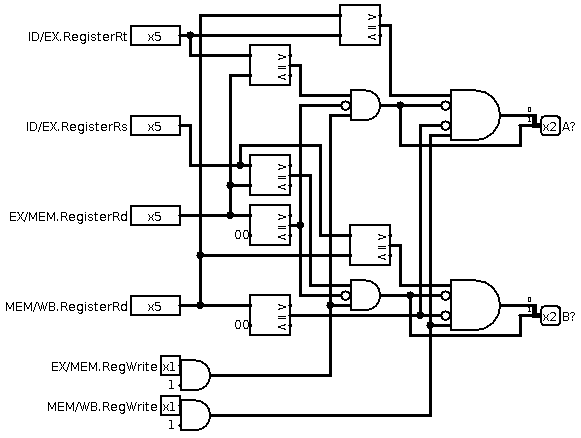
\includegraphics[width=1\textwidth]{forwarding_unit.png}
\end{center}
\caption{Fremsendingsenhed}
\label{fig:fu}
\end{figure}

\section{Fareafsløringsenhed}
Ligesom fremsendingsenheden er vores fareafsløringsenhed (se Figur \ref{fig:hdu})
implementeret fra pseudokoden i COD (s. 372). Det er vigtigt at bemærke at 
det eneste enheden foretager sig er at stalle -- informationen om hvorvidt de 
enkelte jump-instruktioner flusher pipeline-registre eller ej har vi flyttet
ud i hver enkelt pipeline, som så modtager en flush-bit fra instruktionen. 

Fareafsløringsenheden sammenligner rs- og rt-registrene i IF/ID og ID/EX. Hvis
to af dem er ens og ID/EX.MemRead-bitten er høj, sender fareafsløringsenheden
en stall-bit ud i systemet. Stall-bitten sendes til programtælleren, hvor den 
benyttes til at (disable) skrivning. Den sendes også til en or-gate hvis 
funktion er at flushe ID/EX-pipelinen. 

\begin{figure}[htb]
\begin{center}
\leavevmode
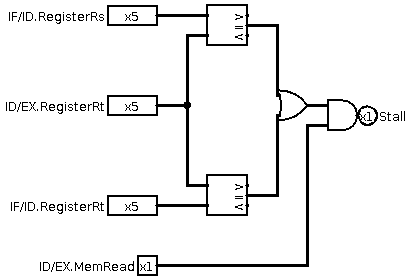
\includegraphics[width=1\textwidth]{hazard_detection_unit.png}
\end{center}
\caption{Fareafsløringsenhed}
\label{fig:hdu} 
\end{figure}

\section{Jump-instruktioner}

\subsection{Jump}
Når jump-bitten i kontrollen er sat (enten i IF/ID eller ID/EX) flusher vi 
instruktionerne i IF/ID, og sender jump-bitten til en mux som vælger imellem
at sende JumpAddr og den sædvanlige inkrementerede værdi til programtælleren.
Denne mux tager også højde for input fra hopforudsigelsesenheden. 

\subsection{Jump and link}
Vi har ændret kontrollogikken for jal-instruktionen så vi, såfremt
jal-bitten er sat, allerede vælger register \$31 i afkodningsstadiet
 -- vi sender \$31 med som instruktionens rd-felt i resten af kredsløbet,
hvor det bruges som signal til fremsendingsenheden. Såfremt jal-bitten 
er sat flusher vi også IF/ID. 

\subsection{Jump register og Branch on equal}
Logikken til håndtering af både jr- og beq-instruktionerne har vi 
placeret i en separat enhed ved navn Jump and Branch Execution Unit. Disse to 
instuktioners implementering er nærmere beskrevet under afsnittet
om hopforudsigelse. 

\section{Hopforudsigelse}
Vi har ikke foretaget nogen ændringer af selve den hopforudsigelsestabel der er 
blevet udleveret til opgaven. Vi sender dens tre output (Tag, Target, P) til 
hopgætteenheden - (se Figur \ref{fig:bgu}) det er en enhed vi har implementeret ud
 fra den udleverede C-kode i opgaveformuleringen. Hopgættenheden sammenligner 
således Tag-signalet med bits 7-31 af programtælleren (i vores tilfælde PC + 4)
 og forudsigelsen (P) med hhv. Weakly og Strongly taken-værdierne. Hvis 
forudsigelsen matcher en af disse, og Tag-signalet matcher PC'en, bliver 
outputtet fra hopgætteenheden sat.

\begin{figure}[htb]
\begin{center}
\leavevmode
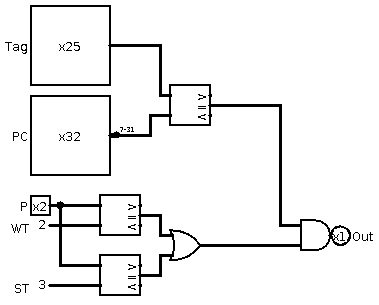
\includegraphics[width=1\textwidth]{branch_guessing_unit.png}
\end{center}
\caption{Hopgætteenhed}
\label{fig:bgu} 
\end{figure} 

\paragraph{}
I modsætning til den udleverede kode indeholder vores hopgætteenhed ikke 
signalet changePc. Vi har kunnet fjerne dette signal grundet den mux vi har 
sat til at vælge imellem de forskellige hop-adresser der sendes til 
programtælleren. Skulle en beq forekomme umiddelbart efter en jump-instruktion
vil muxen vælge jump-adressen som den værdi der sendes til PC. Dette gælder
også for jal-instruktionen. 

\subsection{Hopudførselsenheden}
I hopudførelsesenhedens (se Figur \ref{fig:jabe}) øverste segment af to mucer
\footnote{Nominativ pluralis af ordet 'mux'} undersøges ALUcontrol-outputtet 
(i tilfælde af jr) og hhv. Branch og ALUzero (i tilfælde af beq) og den værdi 
der sendes som opdatering til PC'en besluttes på baggrund af resultatet. Når 
der udføres en beq-instruktion skrives den nye programtæller også videre i 
Target-outputtet (der kan også skrives til Target i tilfælde af en jr-instruktion,
men eftersom Branch-bitten i så fald ikke vil være sat vil dette ikke blive registreret).

\paragraph{}
Hopudførelsesenheden tager også hånd om flushing i tilfælde af kontrolfarer
ved udførelse af hop. Her sammenlignes den nuværende Target-værdi med den
der bliver udregnet i tilfælde af beq-instruktioner, og resultatet
sendes til en PLA sammen med ALUkontrollen, ALUzero- og Branch-bitten og 
det hop-gæt der er blevet sendt fra Hopforudsigelsestabellen. Outputtet
fra PLA'en bestemmer hvorvidt IF/ID og ID/EX flushes, samt hvorvidt det er
jr-adressen, beq-adressen eller PC + 4 der skal sendes til programtælleren. 
Sandhedstabellen for PLA'ens udregninger forefindes nedenfor:

\begin{table}[htb]
    \hspace{1cm}
    \begin{tabular}{ccc|cl}
        Guess & Equal & Branching & Flush \& Send back & \\ \cline{1-4}
        0 & 0 & 0 & 0 & \color{gray}Ingen branching og \\
        &   &   &   & \color{gray}          rigtigt gæt.\\
        0 & 0 & 1 & 1 & \color{gray}Beq-adresse sendes \\
        &   &   &   & \color{gray}          tilbage.\\
        0 & 1 & 0 & 0 & \color{gray}Bør kun kunne ske \\
        &   &   &   & \color{gray}           ved støj.\\
        0 & 1 & 1 & 1 & \color{gray}Beq-adresse sendes \\
        &   &   &   & \color{gray}           tilbage.\\
        1 & 0 & 0 & 1 & \color{gray}PC+4 sendes tilbage.\\
        1 & 0 & 1 & 1 & \color{gray}Target og Beq er ikke\\
        &   &   &   & \color{gray}        ens. Vi sender Beq-\\
        &   &   &   & \color{gray}          adressen tilbage.\\
        1 & 1 & 0 & 1 & \color{gray}PC+4 sendes tilbage.\\
        1 & 1 & 1 & 0 & \color{gray}Branching og rigtigt\\
        &   &   &   & \color{gray}           gæt.\\
    \end{tabular}
\end{table} 

\begin{figure}[htb]
\begin{center}
\leavevmode
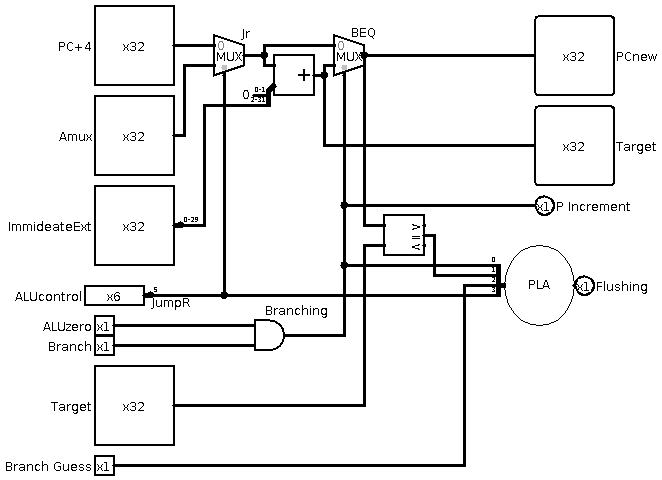
\includegraphics[width=1\textwidth]{jump_and_branch_excecution_unit.png}
\end{center}
\caption{Hopudførelsesenhed}
\label{fig:jabe} 
\end{figure}

\end{document}
